\documentclass{beamer}
%
% Choose how your presentation looks.
%
% For more themes, color themes and font themes, see:
% http://deic.uab.es/~iblanes/beamer_gallery/index_by_theme.html
%
\mode<presentation>

\usetheme{Dresden}
\definecolor{RPISECText}{RGB}{16,16,16}
\definecolor{RPISECHeader}{RGB}{11,200,238}
\definecolor{RPISECGraphic}{RGB}{226,35,27}
\setbeamercolor{title}{fg=RPISECText}
\setbeamercolor{structure}{fg=RPISECGraphic}
\setbeamercolor{frametitle}{fg=RPISECText}
\setbeamercolor{sectiontitle}{fg=RPISECHeader,bg=RPISECText}
\setbeamerfont{title}{series=\bfseries}

\makeatletter
\let\beamer@writeslidentry@miniframeson=\beamer@writeslidentry
\def\beamer@writeslidentry@miniframesoff{%
  \expandafter\beamer@ifempty\expandafter{\beamer@framestartpage}{}% does not happen normally
  {%else
    % removed \addtocontents commands
    \clearpage\beamer@notesactions%
  }
}
\newcommand*{\miniframeson}{\let\beamer@writeslidentry=\beamer@writeslidentry@miniframeson}
\newcommand*{\miniframesoff}{\let\beamer@writeslidentry=\beamer@writeslidentry@miniframesoff}
\makeatother

\AtBeginSection[] {
\miniframesoff
\begin{frame}
  \vfill
  \centering
  \begin{beamercolorbox}[sep=8pt,center,shadow=true,rounded=true]{sectiontitle}
    \usebeamerfont{title}\insertsectionhead\par%
  \end{beamercolorbox}
  \vfill
\end{frame}
\miniframeson
}

\usepackage[english]{babel}
\usepackage[utf8x]{inputenc}

\usepackage[ruled]{algorithm2e}

\title{Counting Triangles in Large Graphs using Randomized Matrix Trace Estimation: an Overview}
\author{Steven Haussmann, Louis Hyde, Peter Wood}
% dated to submit on the 3rd
\date{Dec. 3, 2018}

\begin{document}

\begin{frame}
  \titlepage
\end{frame}

\section{Background}

\subsection{Introduction}

\begin{frame}
    A \textbf{triangle} is a group of three nodes in a graph that are pairwise connected
    
    \begin{itemize}
        \item Alice, Bob, and Charlie are all friends with one another
        \item Three cities are connected by freeways
    \end{itemize}
\end{frame}

\begin{frame}
\begin{itemize}
    \item The number of triangles in a graph provides interesting information:
    
    \begin{itemize}
        \item Clustering coefficient - how likely are nodes to be linked?
    \end{itemize}
    
    \item Iterating over nodes or edges takes $O(\sum_{v\in V} deg(v)^2) \approx O(|E|^2)$ time and is hard to parallelize

    \item Monte Carlo simulation to check if random nodes/edges form a triangle only works for dense graphs
\end{itemize}
\end{frame}

\subsection{The Paper}

\begin{frame}
    We examined a 2010 paper on the subject, \textit{Counting Triangles in Large Graphs using Randomized Matrix Trace Estimation}
    
    \begin{itemize}
        \item Authored by Haim Avron of Tel-Aviv University
    \end{itemize}
\end{frame}

\begin{frame}
    Avron presents a \textit{randomized approach} to triangle counting.
    
    We examine two of his proposed algorithms.
\end{frame}

\section{Algorithm}

\subsection{Trace Estimation}

\begin{frame}{Randomized Trace Estimation}
\begin{itemize}
    \item $A$ is the adjacency matrix
    \item $x$ is a vector whose entries are independent random variables with expectation 0 and variance 1
    \item Calculate $y=Ax$
    \item Then $y^T A y = (x^T A) A (Ax) = x^T A^3 x$ approximates $tr(A^3)$
    
\end{itemize}
\end{frame}

\begin{frame}{Randomized Trace Estimation, cont'd}
\begin{itemize}
    \item $\mathbb E (x^T A x) = \sum_{i=0}^n \sum_{j=0}^n \mathbb E (x_i A_{ij} x_j)$
    \item Since $\mathbb E x_i = 0$, $\mathbb E (x_i x_j) = 0$ for $i\neq j$, so $\sum_{i\neq j} \mathbb E(x_i A_{ij} x_j) = 0$
    \item Since $\mathbb E (x_i^2) = \mathbb E(x_i^2) + Var(x_i) = 1$, $\mathbb E(x_i A_{ii} x_i) = A_{ii}$
    \item Thus $\mathbb E (x^T A x) = \sum_{i=0}^n A_{ii} = Tr(A)$
\end{itemize}
    
\end{frame}

\subsection{Algorithm}

% we can probably just re-write the algorithm section from the paper here

\begin{frame}
    Two variants of the same algorithm were presented by the author:
    
    \begin{itemize}
        \item \texttt{TraceTriangleN} (normal RVs)
        \item \texttt{TraceTriangleR} (Rademacher RVs)
    \end{itemize}
    
\end{frame}
\begin{frame}[fragile]
    \texttt{TraceTriangleN}
    \begin{algorithm}[H]
        \SetAlgorithmName{TraceTriangleN}
        \KwData{$G$, an undirected graph of $N$ nodes, and $\gamma$}
        \KwResult{$\Delta$, the estimated number of triangles}
        Form an adjacency matrix $A \in R^{n \times n}$\;
        $M \leftarrow \lceil \gamma \ln^2 n \rceil$\;
        $i \leftarrow 0$\;
        \While{$i < M$} {
            $x \leftarrow (x_k)$ where $x_i \sim N(0,1)$ ($x_i$ are i.i.d.)\;
            $y \leftarrow Ax$\;
            $T_i \leftarrow (y^T A y)/6$\;
            $i \leftarrow i + 1$\;
        }
        $\Delta \leftarrow \frac{1}{M} \sum_{i=1}^{M} T_i$\;
    \end{algorithm}
\end{frame}


\begin{frame}
    Variants of the algorithm:
    
    \begin{itemize}
        \item Multiple ways to sample $x$
        \item Author notes that $N(0,1)$ gives the best bound
        \item Rademacher approach is better for implementation, however
        \item Also theoretically has a better estimator of the trace
    \end{itemize}
    
\end{frame}

\begin{frame}
In summary:
    \begin{itemize}
     \item Compute the average of $M$ samples
     \item Samples can be taken in parallel
     \item Experimental results suggest $M = \lceil \gamma \ln^2 |V| \rceil$
    \end{itemize}
\end{frame}

\section{Analysis}

\subsection{Theoretical Results}

%% TODO: explain runtime
\begin{frame}{Speedup}
    \begin{itemize}
        \item Any exact algorithm has to involve matrix multiplication, which is na\"ively $O(|V|^3)$
        \item Better multiplication algorithms live somewhere above $O(|V|^2)$
        \item \texttt{TraceTriangle} requires $O(|E|)$ time for each sample
        \begin{itemize}
            \item Requires $A \times x$ for each iteration, which would make it $O(|V|^2)$ but if $A$ is sparse, this could be made $O(|E|)$
        \end{itemize}
        \item $\lceil \gamma \log^2(|V|) \rcel$ samples are needed
        \item Total runtime: $O(\gamma |E| \log^2 |V| )$
    \end{itemize}
\end{frame}

\begin{frame}
    Avron describes $(\varepsilon, \delta)$ bounds on error.
    
    \begin{itemize}
        \item Depends on $\rho(G)$ - the \textit{eigenvalue triangle sparsity} of the graph.
        \item $\rho(G) = \frac{\sum_{i=1}{n} |\lambda_i^3|}{6 \Delta(G)}$
        \item Very small triangle counts and very large eigenvalues cause large error bounds
        \item $\gamma$ required for $\varepsilon = 0.05$, $\delta = 0.05$ is enormous
        \item Author notes that small $\gamma$ works well \textit{in practice} for commonly encountered graphs.
    \end{itemize}
\end{frame}

\begin{frame}{Random Bits}
    \begin{itemize}
        \item \texttt{TraceTriangleN} requires $n$ random numbers per step
        \item $O(\gamma \log^2 |V|)$ total bits
        \item \texttt{TraceTriangleR} is similar, requiring $n$ random bits
        \item Avron proposed a third algorithm requiring significantly fewer; not examined here
    \end{itemize}
    Random number generation may seem trivial, but becomes difficult in massively parallel situations
\end{frame}

\begin{frame}{Scalability}
    \texttt{TraceTriangleN} is \textit{embarrassingly parallel}
    \begin{itemize}
        \item Each iteration is independent of all other iterations
        \item Can easily farm out to many processors
    \end{itemize}
    The algorithm can also be streamed.
    \begin{itemize}
        \item One pass requires $O(|V| \log^2 |V|)$ memory
        \item Less memory is consumed if several passes are made
    \end{itemize}
\end{frame}

\subsection{Empirical Results}

\begin{frame}
    We evaluated the performance of \texttt{TraceTriangleN} and \texttt{TraceTriangleR} in three situations:
    
    \begin{itemize}
        \item Runtime on graphs of varying size
        \item Runtime and variance of results with varying $\gamma$
        \item Variance and error of results with varying triangle sparsity
    \end{itemize}
\end{frame}

\begin{frame}
    Notes:
    
    \begin{itemize}
        \item The exact algorithm directly computes $\textrm{Tr}(A^3)$
        \item \texttt{TraceTriangleN} and \texttt{TraceTriangleR} are not parallelized
        \item $\gamma = 1$ unless otherwise noted
        \item Sparse matrix multiplication was not performed (increasing runtime)
    \end{itemize}
\end{frame}

\begin{frame}{Runtime}
    We evaluated runtime for graphs of varying size.
    
    \begin{itemize}
        \item $|V| = 1000, 2000, \ldots, 10000$
        \item $\gamma = 1$
        \item 25 trials
    \end{itemize}
\end{frame}

\begin{frame}
    \begin{figure}
        \centering
        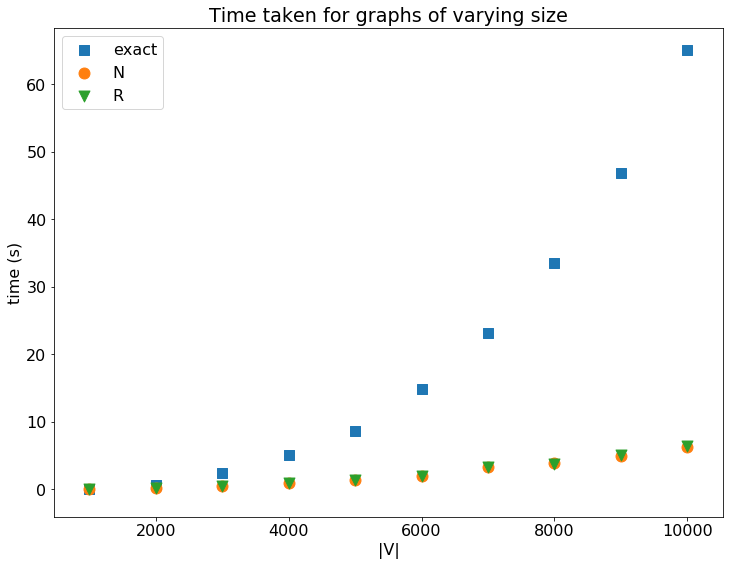
\includegraphics[width=0.7\linewidth]{figs/size-time.png}
        \caption{Exactly computing $\textrm{Tr}(A^3)$ proves to be far more expensive than the randomized approach.}
        \label{fig:size-time}
    \end{figure}
\end{frame}

\begin{frame}
    \begin{figure}
        \centering
        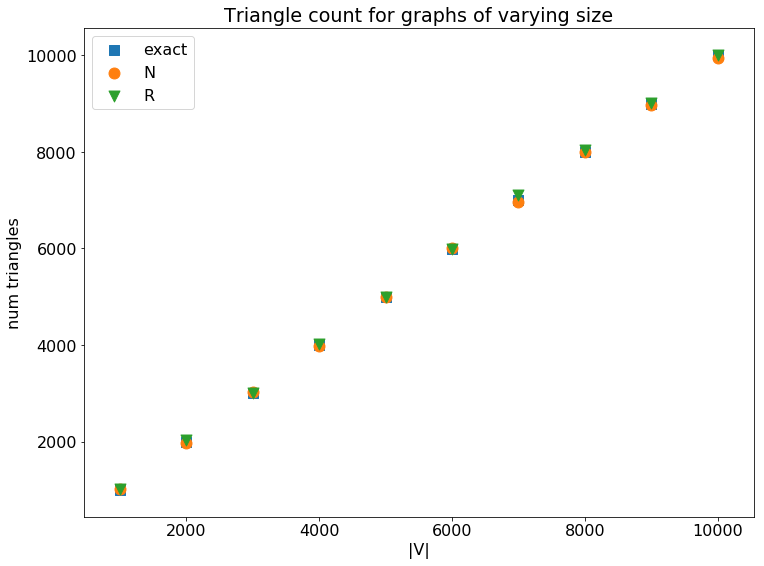
\includegraphics[width=0.7\linewidth]{figs/size-count.png}
        \caption{$\gamma = 1$, but values presented are the average of 25 trials (similar to letting $\gamma = 25$). We examine accuracy more closely next.}
        \label{fig:size-time}
    \end{figure}
\end{frame}

\begin{frame}{Gamma}
    We examined the variance and average absolute percent error, where:
    
    \begin{itemize}
        \item $|V| = 1000$
        \item $A$ is tridiagonal
        \item $\gamma = 1, 2, \ldots, 10$
        \item 100 trials were performed for each value of $\gamma$
    \end{itemize}
\end{frame}

\begin{frame}
    \begin{figure}
        \centering
        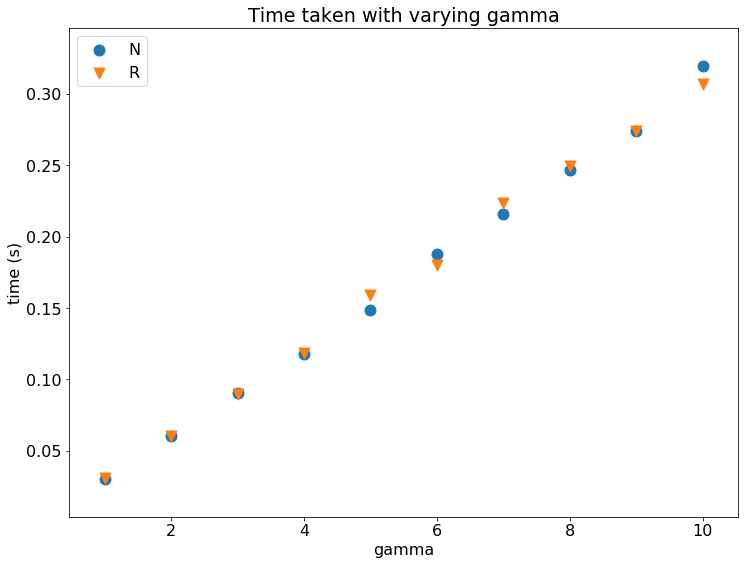
\includegraphics[width=0.7\linewidth]{figs/gamma-time.png}
        \caption{As expected, time taken scales linearly with $\gamma$}
        \label{fig:gamma-time}
    \end{figure}
\end{frame}

\begin{frame}
    \begin{figure}
        \centering
        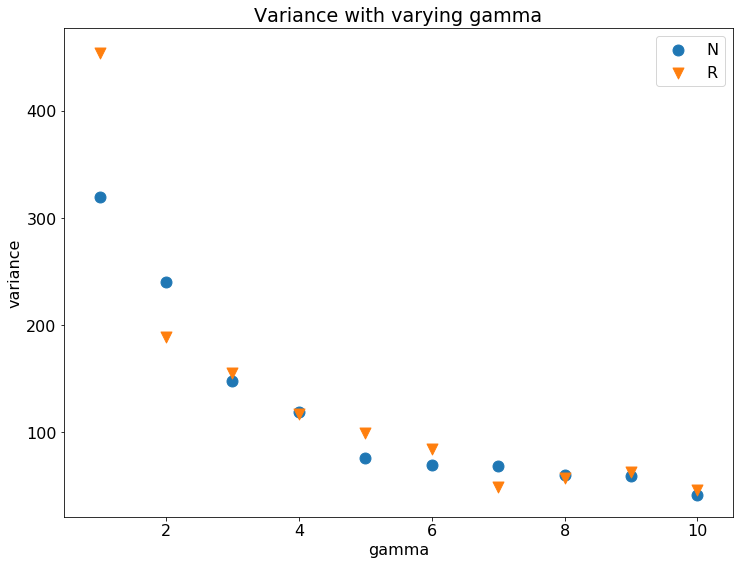
\includegraphics[width=0.7\linewidth]{figs/gamma-variance.png}
        \caption{Variance declines as $\gamma$ increases. Note the apparent noise, even with 100 trials.}
        \label{fig:gamma-variance}
    \end{figure}
\end{frame}

\begin{frame}
    \begin{figure}
        \centering
        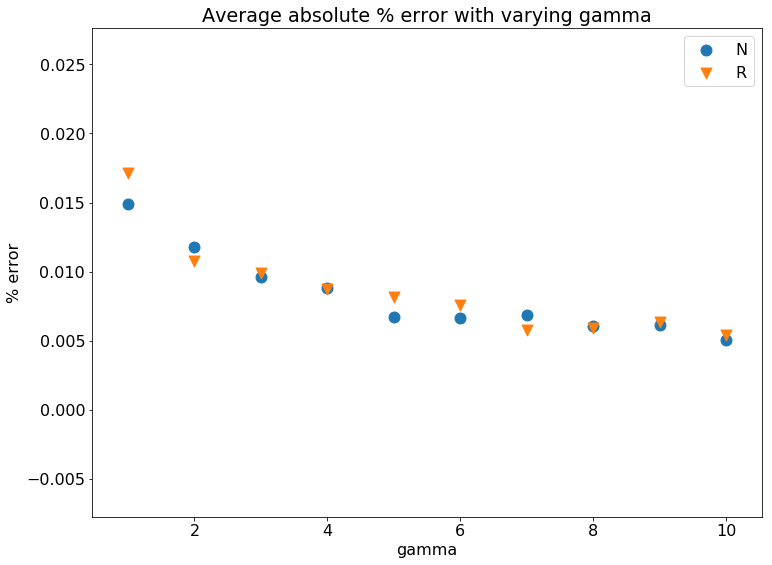
\includegraphics[width=0.7\linewidth]{figs/gamma-error.png}
        \caption{Average absolute percent error also declines.}
        \label{fig:gamma-error}
    \end{figure}
\end{frame}

\begin{frame}{Sparsity}
    We examined the variance and average absolute percent error, where:
    
    \begin{itemize}
        \item $|V| = 100$
        \item $\max(\Delta(G)) = 100 \times 99 \times 98 / 6 = 161700$
        \item $A$ has $n$ number of triangles added randomly:
        \begin{itemize}
            \item Select random distinct $i,j,k$
            \item Connect vertices $i,j,k$ together
        \end{itemize}
        \item $n = [2^0, 2^\frac{1}{2}, 2^1, \ldots, 2^{20}]$
        \item $\gamma = 1$
        \item 25 trials were performed for each value of $n$
    \end{itemize}
\end{frame}

\begin{frame}
    \begin{figure}
        \centering
        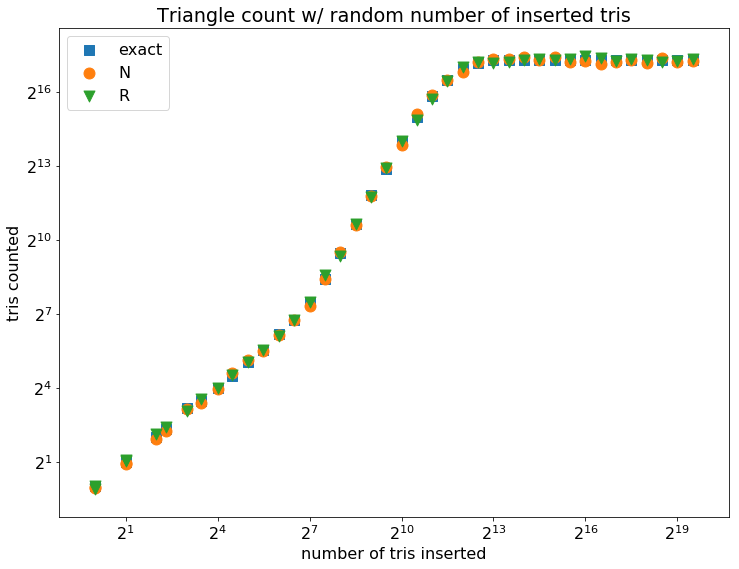
\includegraphics[width=0.7\linewidth]{figs/number-count.png}
        \caption{Note how each added triangle may actually create more than one triangle, and how the graph becomes ``saturated''}
        \label{fig:number-count}
    \end{figure}
\end{frame}

\begin{frame}
    \begin{figure}
        \centering
        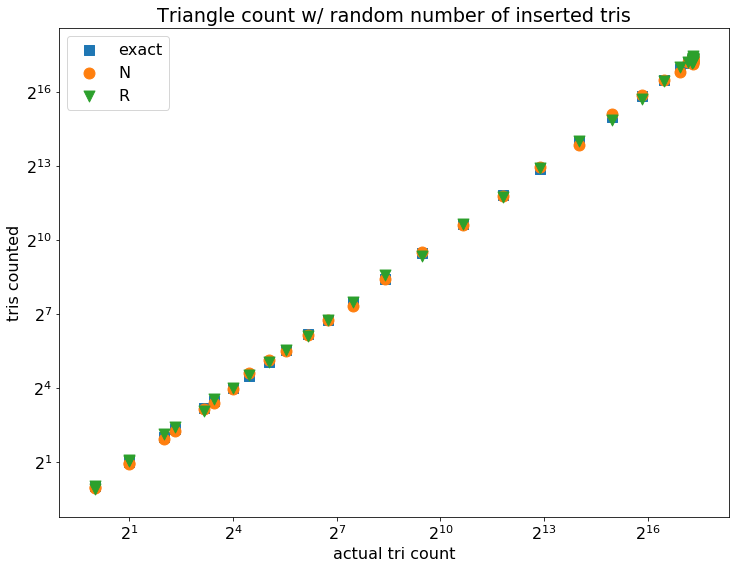
\includegraphics[width=0.7\linewidth]{figs/number-actual.png}
        \caption{Replacing the x-axis with the \textit{actual} number of triangles gives a straigther line.}
        \label{fig:number-count}
    \end{figure}
\end{frame}


\begin{frame}
    \begin{figure}
        \centering
        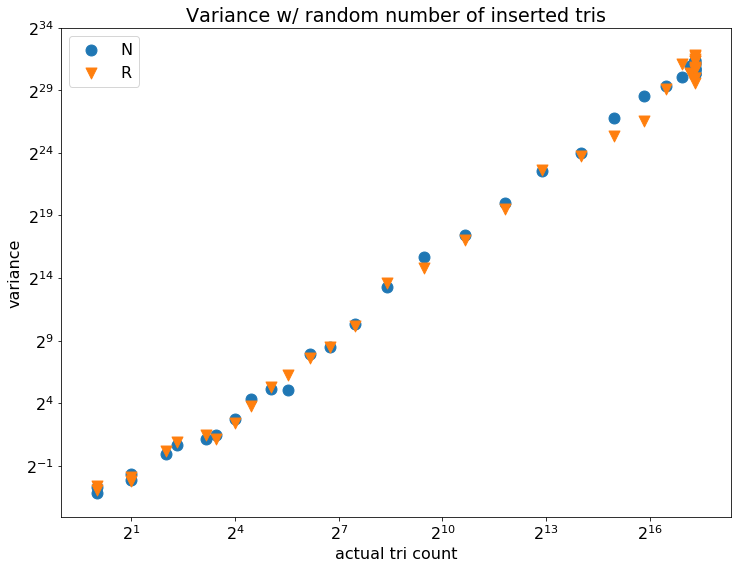
\includegraphics[width=0.7\linewidth]{figs/number-variance.png}
        \caption{The variance grows with the number of triangles, as expected. A slight dip is observed in the sparser regions.}
        \label{fig:number-variance}
    \end{figure}
\end{frame}

\begin{frame}
    \begin{figure}
        \centering
        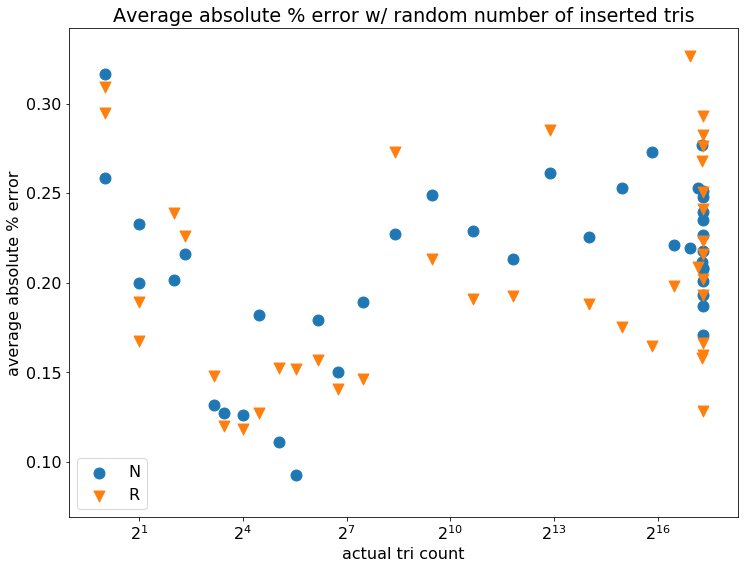
\includegraphics[width=0.7\linewidth]{figs/number-error.png}
        \caption{The average absolute percent error is lowest when the graph is sparse (but not \textit{too} sparse). Note that the repeated trials for a completely full graph gave widely varying results.}
        \label{fig:number-error}
    \end{figure}
\end{frame}

\section{Conclusions}

\subsection{Conclusions}

\begin{frame}
    Objective
    \begin{itemize}
        \item \texttt{TraceTriangle} offers significant speedup over the na\"ive approach
        \item Parallelization is straightforward, although bandwidth is a concern.
        \item Accuracy is reasonable
        \begin{itemize}
            \item Being an unbiased estimator means many trials can be averaged
        \end{itemize}
        \item Somewhat questionable theoretical basis - low values of $\gamma$ don't provide strong guarantees, but do work on real data.
    \end{itemize}
\end{frame}

\begin{frame}
    Subjective
    \begin{itemize}
        \item \textit{Counting Triangles} has over 50 citations
        \item Builds on both deterministic and randomized work
        \item 2010 paper, so work has been done since publication
    \end{itemize}
\end{frame}

\end{document}
